\documentclass[11pt,a4paper]{article}

% ---------------------------------------------------------------------------
% An exact oscillatory instability in a minimal Type II autocatalytic core
% with linear degradation.
%
% Author metadata: set the three macros below before submission.
% ---------------------------------------------------------------------------
\newcommand{\PaperAuthor}{}
\newcommand{\PaperAffiliation}{}
\newcommand{\PaperDate}{14 September 2026}

\usepackage[T1]{fontenc}
\usepackage[utf8]{inputenc}
\usepackage{lmodern}
\usepackage{microtype}
\usepackage[a4paper,margin=1.05in]{geometry}
\usepackage{amsmath,amssymb,amsthm,mathtools}
\usepackage{graphicx}
\usepackage{float}
\usepackage{booktabs}
\usepackage{array}
\usepackage{enumitem}
\usepackage{xcolor}
\usepackage{listings}
\usepackage{tikz}
\usetikzlibrary{arrows.meta}
\usepackage[obeyspaces,spaces]{url}
\usepackage[colorlinks=true,linkcolor=blue!55!black,citecolor=blue!55!black,urlcolor=blue!55!black]{hyperref}

\hypersetup{pdftitle={An exact oscillatory instability in a minimal Type II autocatalytic core with linear degradation},
  pdfsubject={A source-minimal Type II autocatalytic core whose unique positive stationary state is unstable under strictly positive linear degradation},
  pdfkeywords={autocatalysis, autocatalytic cores, chemical reaction networks, mass action, Hurwitz stability, oscillatory instability, degradation, Lean 4}}

\setlist{itemsep=2pt,topsep=3pt}
\setlength{\emergencystretch}{1.5em}

\lstdefinelanguage{Lean}{
  morekeywords={theorem,def,structure,inductive,namespace,end,import,by,intro,exact,constructor},
  sensitive=true,
  morecomment=[l]{--},
  morestring=[b]",
}
\lstset{
  language=Lean,
  basicstyle=\ttfamily\small,
  keywordstyle=\bfseries,
  commentstyle=\itshape\color{black!60},
  columns=fullflexible,
  keepspaces=true,
  breaklines=true,
  frame=single,
  framerule=0.3pt,
  xleftmargin=1em,
  xrightmargin=1em,
  extendedchars=true,
  literate={≤}{{$\le$}}1 {ℕ}{{$\mathbb{N}$}}1 {ℝ}{{$\mathbb{R}$}}1 {ℂ}{{$\mathbb{C}$}}1 {→}{{$\to$}}1 {∀}{{$\forall$}}1 {∃}{{$\exists$}}1 {≠}{{$\neq$}}1 {∧}{{$\wedge$}}1 {¬}{{$\neg$}}1
}

\theoremstyle{plain}
\newtheorem{theorem}{Theorem}[section]
\newtheorem{proposition}[theorem]{Proposition}
\newtheorem{lemma}[theorem]{Lemma}
\newtheorem{corollary}[theorem]{Corollary}
\newtheorem{question}[theorem]{Question}
\theoremstyle{definition}
\newtheorem{definition}[theorem]{Definition}
\theoremstyle{remark}
\newtheorem{remark}[theorem]{Remark}

\numberwithin{equation}{section}

\newcommand{\R}{\mathbb{R}}
\newcommand{\C}{\mathbb{C}}
\newcommand{\N}{\mathbb{N}}
\newcommand{\one}{\mathbf{1}}
\newcommand{\diag}{\operatorname{diag}}
\renewcommand{\Re}{\operatorname{Re}}
\renewcommand{\Im}{\operatorname{Im}}
\newcommand{\II}{\mathrm{II}}
\newcommand{\Top}{\mathrm{(Top)}}
\newcommand{\iu}{\mathrm{i}}
\DeclareUrlCommand\lean{\urlstyle{tt}}

\title{An exact oscillatory instability in a minimal Type $\II$\\ autocatalytic core with linear degradation}
\author{\PaperAuthor\\ \PaperAffiliation}
\date{\PaperDate}

\begin{document}
\maketitle

\begin{abstract}
The minimal autocatalytic cores of diluted reaction networks were classified by Nandan, Nghe and Unterberger into five families. For the reversible mass-action extension of a core with linear degradation of every species it is known that the positive stationary state, when it exists, is unique, and that it is locally asymptotically stable whenever the degradation constants are small enough. We show that the unique positive stationary state of a minimal core need not be stable for larger degradation. We construct a source-minimal Type $\II_3$ core with seven species, unit stoichiometric coefficients, and a single intermediate on one of the three return paths permitted by the classification, together with strictly positive rational reversible rate constants and strictly positive rational degradation constants, whose unique positive stationary state has the exact Jacobian eigenvalues $1\pm8\iu$. The certificate consists of a stationary flux balance and two integer matrix identities; no root isolation and no numerical eigenvalue computation enters the proof. The stationary state is therefore Hurwitz unstable, the unstable mode is oscillatory, and instability persists on an open set of admissible parameters. We explain the mechanism: contracting the return intermediate at zero frequency gives a Hurwitz-stable six-dimensional matrix, so the instability is carried by the frequency-dependent response of the internal species, and it is invisible in the logarithmically scaled Jacobian, which is stable. We also describe the method that produced the exact certificate, in which a prescribed rational modal shape turns the design of an exact complex eigenvalue at a positive stationary state into a linear feasibility problem. Source membership, stationarity, the Fr\'echet derivative of the full seven-dimensional vector field, the eigenpair and the spectral conclusion are verified in Lean~4 against Mathlib with warnings treated as errors and no unproved declarations. The example does not settle the stability of the six-species cores without internal return species, and it does not assert a periodic orbit.
\end{abstract}

\noindent\textbf{Keywords.} autocatalysis; autocatalytic cores; chemical reaction networks; mass-action kinetics; Hurwitz stability; oscillatory instability; degradation; formal verification.

\medskip
\noindent\textbf{MSC 2020.} 92C42, 80A30; secondary 34D20, 15A18, 68V20.

\section{Introduction}\label{sec:intro}

A reaction network is autocatalytic when a set of species can amplify itself from an external food supply. The question of which small motifs can do this goes back to the autocatalytic sets of Kauffman~\cite{Kau86} and the reflexively autocatalytic food-generated sets of Hordijk and Steel~\cite{HS04}, and was given a stoichiometric foundation by Blokhuis, Lacoste and Nghe~\cite{BLN20}. In the \emph{diluted regime}, where every reaction consumes a single molecule of the autocatalytic species, Unterberger and Nghe~\cite{UN22} showed that stoichiometric autocatalysis is equivalent to a topological condition $\Top$ on the split graph of the network. Nandan, Nghe and Unterberger~\cite{NNU26} classified the minimal networks satisfying $\Top$, the \emph{autocatalytic cores}, into five families, and studied the mass-action dynamics of their reversible extensions under linear degradation of every species.

The dynamical picture of a core that has emerged from~\cite{NNU26} and the two companion papers~\cite{TypeIIpos,TypeIImixed} is one of rigidity. With strictly positive reversible rate constants, every classified core has at most one positive stationary state, whether degradation is absent, strictly positive, or mixed~\cite[Theorems~4.1 and~5.2]{NNU26}, \cite{TypeIIpos}, \cite[Theorem~1.1]{TypeIImixed}. The stationary Jacobian is nonsingular at every positive stationary state, so a positive state can never be lost by collision with another positive state. Without degradation the reversible extension is detailed balanced in the sense of Horn and Jackson~\cite{HJ72}, its unique positive state is locally asymptotically stable, and by openness of the Hurwitz condition the same holds for every sufficiently small degradation vector~\cite[Proposition~8.4]{TypeIImixed}. The abstract of~\cite{NNU26} draws the natural conclusion that the stationary point of a core is likely to be robust under perturbation, and that more complex behaviour is to be expected only from additional nonlinear couplings between cores.

This paper shows that for the Type $\II$ family the last step of that picture does not extend from small to arbitrary degradation. The question is whether the unique positive stationary state of a source-minimal core is Hurwitz stable for \emph{every} choice of positive reversible rate constants and positive degradation constants. For the Type $\II_3$ cores in the form permitted by the classification, which allows each return link of the fork cycle to be a finite reversible path of unit reactions, the answer is no, and the failure is already present with unit stoichiometric coefficients, a single internal species, and strictly positive degradation of every species.

\subsection*{The example}
Order the species as $(A_0,B_0,A_1,B_1,A_2,B_2,C)$. The forward reactions are
\begin{equation}\label{eq:network}
\begin{aligned}
&A_0\to B_0+B_2,\qquad A_1\to B_1+B_0,\qquad A_2\to B_2+B_1,\\
&B_1\to A_2,\qquad B_2\to A_0,\qquad B_0\to C,\qquad C\to A_1 .
\end{aligned}
\end{equation}
Contracting the two-step path $B_0\to C\to A_1$ to a single reaction $B_0\to A_1$ leaves the cyclic backbone $A_0\to B_0\to A_1\to B_1\to A_2\to B_2\to A_0$ with three fork reactions, each of which produces its successor on the backbone together with one earlier backbone species: the separated unit Type $\II_3$ core of~\cite{NNU26}. The species $C$ is the one internal species of a finite unit return path, which the classification permits. We consider the reversible mass-action extension of~\eqref{eq:network}, in which every reaction has a strictly positive forward and reverse rate constant, and every one of the seven species, including $C$, degrades linearly with a strictly positive constant.

\begin{theorem}[Main theorem]\label{thm:main}
The network~\eqref{eq:network} is a source-minimal Type $\II_3$ autocatalytic core with unit weights and one subdivided return path. There exist strictly positive rational reverse and forward rate constants for its seven reversible reactions and strictly positive rational degradation constants for its seven species, given explicitly in Section~\ref{sec:data}, such that the reversible mass-action extension has exactly one positive stationary state $x$, and the Jacobian of the full seven-dimensional vector field at $x$ has the eigenvalues $1\pm8\iu$. In particular $x$ is not Hurwitz stable, and it is an unstable equilibrium of the nonlinear dynamics, with an oscillatory unstable mode.
\end{theorem}

The parameters are given as integers, and the proof of the spectral statement consists of a stationary flux balance $N(p-q)=e$ and two integer matrix identities, $Hu=X(u-8v)$ and $Hv=X(8u+v)$, for explicit integer vectors $u,v$ (Section~\ref{sec:mode}). No characteristic polynomial is expanded, no root is isolated, and no floating-point eigenvalue enters the argument. The identities are short enough to be checked by hand from the tables in Section~\ref{sec:data}, and they have been checked by the Lean~4 proof assistant against the literal source normal form used in the companion papers, so that the example is docked to the same formal notion of ``source-minimal Type $\II_\ell$ core'' for which the uniqueness theorems were proved (Section~\ref{sec:formal}).

\subsection*{Why this is not a routine numerical counterexample}
Three features of the problem made the example harder to find than its final form suggests, and each has a general lesson.

First, the natural coordinates for the search are not rate constants but \emph{stationary coordinates}: the forward and reverse fluxes $p,q$, the degradation fluxes $e$ and the concentrations $x$ at the stationary state, subject only to the balance $N(p-q)=e$ and to positivity. Every positive stationary state of every rate assignment arises exactly once in these coordinates, and rate constants are recovered by division (Lemma~\ref{lem:coverage}). This is the convex parametrisation of stoichiometric network analysis in the sense of Clarke~\cite{Clarke1980}, specialised to cores. In these coordinates the Jacobian factorises as $A=HX^{-1}$, where $H$ depends only on $(p,q,e)$ and $X=\diag(x)$ (Lemma~\ref{lem:jacobian}). The stability question is therefore a question about the pencil $\lambda X-H$, not about $H$ alone, and the two questions have different answers here: for our parameters, $H$ is numerically Hurwitz stable while $A=HX^{-1}$ is not. A search at fixed concentrations, or an argument about the logarithmically scaled Jacobian, cannot see the instability.

Second, the instability is carried by the internal species $C$ of the return path, but not in the way a stationary reduction can detect. At stationarity a reversible unit path is exactly equivalent to a single reversible reaction with endpoint leakage, and this reduction is the basis of the uniqueness proofs~\cite{TypeIIpos,TypeIImixed}. Dynamically the reduction is only the zero-frequency value of a first-order transfer function: eliminating $C$ at complex frequency $s$ contributes $J_{ri}(s-L)^{-1}J_{ir}$ to the retained six-dimensional block, and at $s=0$ this is the stationary Schur complement (Section~\ref{sec:mechanism}). For our parameters the stationary Schur complement is numerically Hurwitz stable; the growing mode has frequency $8$ and the internal relaxation rate of $C$ is about $6.1$, so the phase lag of the return response is substantial and the six-dimensional contraction misses the instability entirely. A stable internal block coupled to a stable contracted block can still be unstable.

Third, exact certification does not require root isolation. Once a numerical unstable mode is in hand, one may \emph{prescribe} a rational modal shape $w$ and a rational eigenvalue $\lambda$ and ask for stationary coordinates realising them. The equation $Hw=\lambda Xw$ is linear in $(e,q,x)$ at fixed $N$ and $w$, and the constraints $e,q,x>0$, $p=q+N^{-1}e>0$ are linear too, so exactification is a small linear feasibility problem (Proposition~\ref{prop:linear}). The rational vertex of that problem, rounded to a modal vector with denominator $200$, is the certificate of Section~\ref{sec:data}. This is why the proof can consist of two integer identities rather than a seventh-degree Hurwitz determinant.

\subsection*{Scope}
Theorem~\ref{thm:main} disproves universal Hurwitz stability for the Type $\II_3$ cores in the form admitted by the classification, already with unit weights and strictly positive degradation. It does not settle whether the six-species cores whose return links are single reactions can be unstable; our bounded numerical searches found no unstable case in that subfamily, which is consistent with, but no evidence for, a stability theorem there. It does not assert a periodic orbit or a Hopf bifurcation: the certified statement is an exact eigenpair of the linearisation with positive real part. It does not assert that instability can be reached by varying degradation alone with the reaction rates held fixed, although Section~\ref{sec:discussion} explains why some crossing of the imaginary axis must occur along any continuous branch of positive states connecting the detailed-balanced state at zero degradation to our parameters. The phenomenon is compatible with all the uniqueness results: for these parameters the unstable state is the only positive stationary state, so the network has no stable positive equilibrium at all.

\subsection*{Formal verification}
The closed declaration \lean{TypeIIStability.typeII3_instability_counterexample} is compiled in Lean~4~\cite{dMU21} against Mathlib~\cite{mathlib20}. Its conclusion is a conjunction: the network is an instance of the literal Type $\II_\ell$ source predicate of~\cite{TypeIIpos,TypeIImixed}; the displayed state is positive and stationary in that source model; every rate and concentration is positive; the full seven-dimensional polynomial vector field vanishes at $x$; its Fr\'echet derivative there is the matrix $A$; and $A$ has the nonzero eigenvector $\xi$ with eigenvalue $1+8\iu$, hence is Hurwitz unstable. A second compiled declaration reuses the companion uniqueness theorem to show that $x$ is the only positive stationary state. The linearised-instability theorem for smooth vector fields, the persistence of the instability under perturbation, and the mechanism analysis of Section~\ref{sec:mechanism} are conventional mathematics and are labelled as such.

\subsection*{Organisation}
Section~\ref{sec:setting} fixes the model, the stationary coordinates and the Jacobian factorisation. Section~\ref{sec:network} identifies the network as a source-minimal Type $\II_3$ core. Section~\ref{sec:data} gives the exact parameters and proves stationarity and uniqueness. Section~\ref{sec:mode} proves the eigenpair identities and the instability, and proves Theorem~\ref{thm:main}. Section~\ref{sec:mechanism} explains the mechanism, describes the search, and proves the linear exact-design proposition. Section~\ref{sec:formal} documents the formal verification, and Section~\ref{sec:discussion} discusses open questions.

\section{Setting}\label{sec:setting}

\subsection{Diluted cores and their reversible extensions}
A diluted network on species $X_1,\dots,X_n$ is a set of reactions each consuming exactly one molecule of one species. Its \emph{split graph} has an edge $X_r\to X_i$ whenever some reaction consumes $X_r$ and produces $X_i$. The network is stoichiometrically autocatalytic when some nonnegative flux vector has strictly positive net production of every species; by~\cite{UN22} this is equivalent to $\Top$, the existence of a strongly connected component of the split graph containing a reaction with at least two products in that component. An \emph{autocatalytic core} is a network satisfying $\Top$ that is minimal under chemostatting, that is, under removal of species from the autocatalytic set together with the reactions that then lose their internal reactant~\cite[\S2]{NNU26}. The classification theorem~\cite[Theorem~3.1]{NNU26} lists five families of cores. The Type $\II_\ell$ cores consist of a main cycle carrying $\ell$ cyclically ordered fork reactions, each producing its successor on the cycle with a positive integer multiplicity and, in addition, one earlier species of the cycle with coefficient one. Between consecutive forks the cycle passes through nonfork species; the link from the back target of a fork to that fork is, before contraction, an arbitrary finite reversible \emph{return path} of one-to-one reactions, and source minimality forces every multiplier on a return path to be one~\cite[Lemma~2.4]{TypeIImixed}. In this paper $\ell=3$, all multiplicities are one, the three forks are separated by one nonfork species each, and one of the three return paths has one internal species.

The dynamics is the mass-action dynamics of the \emph{reversible extension}: every reaction $X_r\to\sum_iP_{ir}X_i$ is made reversible with rate constants $k_r^+,k_r^->0$, and every species is given a linear degradation reaction $X_i\to\varnothing$ with constant $d_i>0$. When every species is the reactant of exactly one forward reaction, as is the case for all networks in this paper, we index reactions by their reactant, so that the product matrix $P\in\N^{n\times n}$ and the stoichiometric matrix $N=P-I$ are square. For a concentration vector $z\in\R^n_{>0}$ write $m_r(z)=\prod_iz_i^{P_{ir}}$ for the product monomial of reaction $r$. The species-formation rate is
\begin{equation}\label{eq:field}
F(z)=N\bigl(k_r^+z_r-k_r^-m_r(z)\bigr)_{r=1}^n-\diag(d)\,z ,
\end{equation}
a polynomial vector field on $\R^n$. A positive stationary state is a vector $x\in\R^n_{>0}$ with $F(x)=0$. It is \emph{Hurwitz stable} if every eigenvalue of the Jacobian $DF(x)$ has strictly negative real part, and \emph{Hurwitz unstable} if some eigenvalue has strictly positive real part.

\subsection{Stationary coordinates}
Fix $N$ with $N$ invertible; this holds for every network considered here, and for every separated Type $\II_\ell$ skeleton~\cite[Lemma~6.1]{TypeIImixed}. Given rate constants and a positive stationary state $x$, define the \emph{stationary coordinates}
\begin{equation}\label{eq:coords}
p_r=k_r^+x_r,\qquad q_r=k_r^-m_r(x),\qquad e_i=d_ix_i,\qquad j=p-q .
\end{equation}
Then $p,q,e,x$ are strictly positive, and $F(x)=0$ reads $Nj=e$.

\begin{lemma}[Coverage]\label{lem:coverage}
Let $N$ be invertible. The map $(k^+,k^-,d,x)\mapsto(p,q,e,x)$ of~\eqref{eq:coords} is a bijection from the set of positive rate assignments together with a positive stationary state onto the set
\[
\mathcal S=\{(p,q,e,x)\in\R^{4n}_{>0}:\ N(p-q)=e\},
\]
with inverse $k_r^+=p_r/x_r$, $k_r^-=q_r/m_r(x)$, $d_i=e_i/x_i$. In particular $\mathcal S$ is parametrised by $(x,e,t)\in\R^{3n}_{>0}$ through $j=N^{-1}e$, $q=\max(0,-j)+t$, $p=q+j$.
\end{lemma}

\begin{proof}
Given $(p,q,e,x)\in\mathcal S$, the displayed rates are positive because $x>0$ and $m_r(x)>0$, and substituting them into~\eqref{eq:field} gives $F(x)=N(p-q)-e=0$. Conversely~\eqref{eq:coords} recovers $(p,q,e,x)$ from the rates and the state, and the two constructions are mutually inverse. For the parametrisation, $q>0$ and $p=q+j>0$ hold if and only if $q>\max(0,-j)$ componentwise, and $j=N^{-1}e$ is forced by $Nj=e$.
\end{proof}

\begin{lemma}[The physical Jacobian]\label{lem:jacobian}
With the rates of Lemma~\ref{lem:coverage} held fixed, the derivative of~\eqref{eq:field} at the stationary state $x$ is
\begin{equation}\label{eq:jacobian}
A:=DF(x)=HX^{-1},\qquad H=N\diag(p)-N\diag(q)P^{\mathsf T}-\diag(e),\qquad X=\diag(x).
\end{equation}
Equivalently, since $P=I+N$ and $p=q+j$,
\begin{equation}\label{eq:factor}
H=-N\diag(q)N^{\mathsf T}+N\diag(j)-\diag(e).
\end{equation}
\end{lemma}

\begin{proof}
For each product monomial, $\partial m_r/\partial z_i(x)=P_{ir}m_r(x)/x_i$. Hence the derivative of $z\mapsto k_r^-m_r(z)$ at $x$ has entries $k_r^-m_r(x)P_{ir}/x_i=q_rP_{ir}/x_i$, and the derivative of $z\mapsto k_r^+z_r$ has entries $k_r^+\delta_{ri}=p_r\delta_{ri}/x_i$. Assembling with $N$ and subtracting $\diag(d)=\diag(e)X^{-1}$ gives $A=HX^{-1}$ with the stated $H$. Substituting $P^{\mathsf T}=I+N^{\mathsf T}$ and $\diag(p)=\diag(q)+\diag(j)$ gives~\eqref{eq:factor}.
\end{proof}

\begin{remark}[The pencil and the scaling freedom]\label{rem:pencil}
The eigenvalue problem $A\xi=\lambda\xi$ is equivalent, through $\xi=Xw$, to the generalised problem $Hw=\lambda Xw$ for the \emph{relative} perturbation $w=X^{-1}\xi$, whose $i$-th component is the perturbation of $\log x_i$. The matrix $H$ is the Jacobian of the field in relative coordinates at the point $\one$, and its spectrum is in general different from that of $A$; positivity of $x$ enters the spectral problem as a positive diagonal mass matrix. The first summand of~\eqref{eq:factor} is symmetric negative definite when $N$ is invertible and $q>0$, and the second, $L=N\diag(j)-\diag(e)$, satisfies $L\one=Nj-e=0$; when $j\ge0$ it is a generator-like matrix. Neither observation controls the spectrum of $HX^{-1}$, and the example of this paper has $j>0$, $H$ numerically Hurwitz stable, and $HX^{-1}$ unstable. Finally, multiplying $(p,q,e,x)$ by a common positive constant $c$ leaves $A$, $k^+$ and $d$ unchanged and multiplies $k_r^-$ by $c^{-1}$ for bimolecular reverse reactions and by $1$ for unimolecular ones: it is a change of concentration unit. We use this freedom to present the certificate with integer entries.
\end{remark}

\section{The network and its source structure}\label{sec:network}

\subsection{Reactions, indices and matrices}
Index the species as $(A_0,B_0,A_1,B_1,A_2,B_2,C)=(X_0,\dots,X_6)$ and the reactions by their reactant, in the same order. The reversible reaction pairs are
\begin{equation}\label{eq:reactions}
\begin{array}{lll}
0\colon\ A_0\rightleftarrows B_0+B_2,\qquad& 1\colon\ B_0\rightleftarrows C,\qquad& 2\colon\ A_1\rightleftarrows B_1+B_0,\\
3\colon\ B_1\rightleftarrows A_2,& 4\colon\ A_2\rightleftarrows B_2+B_1,& 5\colon\ B_2\rightleftarrows A_0,\\
6\colon\ C\rightleftarrows A_1,&&
\end{array}
\end{equation}
with forward directions from left to right, together with $X_i\to\varnothing$ for $i=0,\dots,6$. The stoichiometric matrix, with species as rows and reactions as columns, is
\begin{equation}\label{eq:N}
N=\begin{pmatrix}
-1&0&0&0&0&1&0\\
1&-1&1&0&0&0&0\\
0&0&-1&0&0&0&1\\
0&0&1&-1&1&0&0\\
0&0&0&1&-1&0&0\\
1&0&0&0&1&-1&0\\
0&1&0&0&0&0&-1
\end{pmatrix},\qquad P=I+N,
\end{equation}
and the product monomials are
\begin{equation}\label{eq:monomials}
m(z)=(z_1z_5,\ z_6,\ z_3z_1,\ z_4,\ z_5z_3,\ z_0,\ z_2)^{\mathsf T}.
\end{equation}
The three fork reactions $0,2,4$ are unimolecular forward and bimolecular reverse; the four return reactions $1,3,5,6$ are unimolecular in both directions. Figure~\ref{fig:network} shows the split graph.

\begin{figure}[t]
\centering
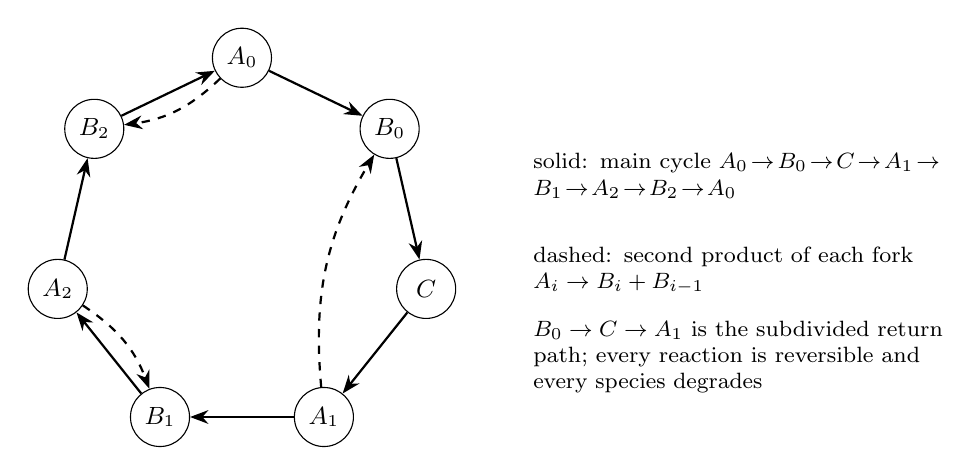
\begin{tikzpicture}[>=Stealth,scale=1.0,
  sp/.style={draw,circle,minimum size=7.5mm,inner sep=0pt,font=\small},
  main/.style={->,thick},
  backe/.style={->,thick,dashed}]
  % seven vertices on a circle, cyclic order A0,B0,C,A1,B1,A2,B2
  \node[sp] (A0) at (90:2.4) {$A_0$};
  \node[sp] (B0) at (90-51.4:2.4) {$B_0$};
  \node[sp] (C)  at (90-102.9:2.4) {$C$};
  \node[sp] (A1) at (90-154.3:2.4) {$A_1$};
  \node[sp] (B1) at (90-205.7:2.4) {$B_1$};
  \node[sp] (A2) at (90-257.1:2.4) {$A_2$};
  \node[sp] (B2) at (90-308.6:2.4) {$B_2$};
  \draw[main] (A0) -- (B0);
  \draw[main] (B0) -- (C);
  \draw[main] (C)  -- (A1);
  \draw[main] (A1) -- (B1);
  \draw[main] (B1) -- (A2);
  \draw[main] (A2) -- (B2);
  \draw[main] (B2) -- (A0);
  \draw[backe] (A0) to[bend left=18] (B2);
  \draw[backe] (A1) to[bend left=18] (B0);
  \draw[backe] (A2) to[bend left=18] (B1);
  \node[font=\footnotesize,text width=5.2cm,align=left] at (6.3,0.9)
    {solid: main cycle $A_0\!\to\!B_0\!\to\!C\!\to\!A_1\!\to\!B_1\!\to\!A_2\!\to\!B_2\!\to\!A_0$};
  \node[font=\footnotesize,text width=5.2cm,align=left] at (6.3,-0.3)
    {dashed: second product of each fork $A_i\to B_i+B_{i-1}$};
  \node[font=\footnotesize,text width=5.2cm,align=left] at (6.3,-1.4)
    {$B_0\to C\to A_1$ is the subdivided return path; every reaction is reversible and every species degrades};
\end{tikzpicture}
\caption{The split graph of the forward network~\eqref{eq:network}. Contracting $B_0\to C\to A_1$ gives the six-species separated unit Type $\mathrm{II}_3$ core; the classification permits the finite unit return path through $C$.}
\label{fig:network}
\end{figure}

\subsection{Membership in the Type \texorpdfstring{$\II_3$}{II\_3} family}
Contracting the path $B_0\to C\to A_1$ to a single reaction identifies the cyclic backbone $A_0\to B_0\to A_1\to B_1\to A_2\to B_2\to A_0$ with fork reactions at $A_0,A_1,A_2$ whose second products are $B_2,B_0,B_1$ respectively. Each fork produces its successor with multiplicity one, its back product has coefficient one, the fork sources and back targets are pairwise distinct (the \emph{separated} weak order), and the three return links $B_2\to A_0$, $B_0\to A_1$, $B_1\to A_2$ have unit multipliers, the second being realised by the two-step path through $C$. This is the separated unit Type $\II_3$ normal form of~\cite{TypeIIpos,TypeIImixed} with return-path depths $(1,2,1)$. It remains to check that the seven-species network is a core, that is, that it satisfies $\Top$ and is minimal.

\begin{proposition}[Source minimality]\label{prop:minimal}
Let $G$ be the split graph of~\eqref{eq:network}, with vertices in cyclic order $(v_0,\dots,v_6)=(A_0,B_0,C,A_1,B_1,A_2,B_2)$. Then $G$ consists of the directed seven-cycle $v_k\to v_{k+1}$ and the three back edges $v_0\to v_6$, $v_3\to v_1$, $v_5\to v_4$, and no proper nonempty vertex set $S$ induces a subgraph in which some fork together with both of its products lies in one strongly connected component. Consequently no proper chemostatted restriction of the network satisfies $\Top$, and the full network does.
\end{proposition}

\begin{proof}
The description of $G$ is read off from $P$. Let $S$ be a proper vertex set and suppose a fork $f\in S$ and its two products $a,b\in S$ lie in a common strongly connected component of the induced subgraph. Since every back edge points to a vertex already visited by the cycle, every directed path in $G$ from a vertex $v_k$ to a vertex $v_m$ with $m\ne k$ must traverse the cycle vertices $v_{k+1},v_{k+2},\dots,v_m$ in order, unless it uses a back edge, and a back edge $v_i\to v_j$ only jumps to an earlier vertex $j<i$ of the current traversal; hence a path from $v_k$ to $v_m$ contains all of $v_{k+1},\dots,v_m$ (indices modulo $7$). For the fork $v_0$ with products $v_1,v_6$, a path from $v_1$ to $v_6$ contains $v_2,\dots,v_5$, so $S\supseteq\{v_0,\dots,v_6\}$. For the fork $v_3$ with products $v_4,v_1$, a path from $v_4$ to $v_1$ contains $v_5,v_6,v_0$, and a path from $v_1$ to $v_3$ contains $v_2$; again $S$ is everything. For the fork $v_5$ with products $v_6,v_4$, a path from $v_6$ to $v_4$ contains $v_0,v_1,v_2,v_3$. In each case $S$ is not proper.

For the consequence, recall that a chemostatted restriction retains a species set $S$ and exactly those reactions whose reactant lies in $S$, with products outside $S$ discarded. Its split graph is the induced subgraph on $S$, and $\Top$ for the restriction asks for a strongly connected component containing a reaction with two products in the component; the only reactions with two products are the three forks. So $\Top$ fails for every proper restriction. The full network satisfies $\Top$ because its split graph is strongly connected (it contains the seven-cycle) and contains a fork.
\end{proof}

The proposition was also confirmed by exhaustive enumeration of the $126$ nonempty proper vertex sets; the enumeration is a transcription check, not part of the proof. Two further structural facts complete the identification.

\begin{proposition}[Autocatalysis and unit return paths]\label{prop:auto}
\begin{enumerate}[label=\textup{(\roman*)}]
\item The forward network~\eqref{eq:network} is stoichiometrically autocatalytic: the flux vector $g=(4,7,4,6,4,6,6)^{\mathsf T}$ has net production $Ng=(2,1,2,2,2,2,1)^{\mathsf T}$, which is strictly positive.
\item The restriction to the return cycle $B_0\to C\to A_1\to B_0$ formed by the return path and the back product of $A_1$ is not stoichiometrically autocatalytic, and the same holds for the one-step return cycles through $B_2$ and $B_1$: on such a restriction every retained reaction consumes one molecule and produces at most one, so the total net production is nonpositive for every nonnegative flux.
\end{enumerate}
\end{proposition}

\begin{proof}
(i) is a direct multiplication with~\eqref{eq:N}. For (ii), the reactions of the return cycle through $C$ are $B_0\to C$, $C\to A_1$ and, restricted to the retained species $\{B_0,C,A_1\}$, the fork $A_1\to B_0$ (the product $B_1$ is discarded). Each is one-to-one, so the sum over retained species of the net production is $\sum_r(\text{products}_r-1)\varphi_r\le0$ for every flux $\varphi\ge0$, and strict positivity at every retained species is impossible.
\end{proof}

Part (ii) is the condition that distinguishes the permitted unit return paths from the weighted return cycles that destroy minimality~\cite[Lemma~2.4]{TypeIImixed}; together with Proposition~\ref{prop:minimal} it is exactly the literal source-minimality predicate of the formal development (Section~\ref{sec:formal}), which requires that no proper weak-stem restriction retains $\Top$ and that no rotated proper return cycle is autocatalytic.

\section{Exact parameters, stationarity and uniqueness}\label{sec:data}

\subsection{The certificate}
The example is specified by the four integer vectors of Table~\ref{tab:data}: the degradation fluxes $e$, the forward fluxes $p$, the reverse fluxes $q$ and the concentrations $x$ at the stationary state, in the sense of~\eqref{eq:coords}. They are not rate constants. The rate constants are defined from them by Lemma~\ref{lem:coverage}:
\begin{equation}\label{eq:rates}
k_r^+=\frac{p_r}{x_r},\qquad k_r^-=\frac{q_r}{m_r(x)},\qquad d_i=\frac{e_i}{x_i}\qquad(r,i=0,\dots,6),
\end{equation}
with $m_r$ as in~\eqref{eq:monomials}. Every entry of Table~\ref{tab:data} is a positive integer and every monomial $m_r(x)$ is a positive integer, so all fourteen reversible rate constants and all seven degradation constants are strictly positive rational numbers.

\begin{table}[t]
\centering\small
\begin{tabular}{@{}crr@{}}
\toprule
$i$ & $e_i$ (degradation flux) & $x_i$ (concentration) \\
\midrule
0 & 119498114558151195430200 & 353827128708175750212000 \\
1 & 50529476583056335199400 & 166846502377565969557740 \\
2 & 102854639051720636741122800 & 33548594408689902229104300 \\
3 & 50529476583056335199400 & 701061232230997648855000 \\
4 & 212440931970968885258100 & 36804829974094783842403500 \\
5 & 50529476583056335199400 & 50529476583056335199400 \\
6 & 50529476583056335199400 & 17556019227313040061617094 \\
\bottomrule
\end{tabular}

\medskip
\begin{tabular}{@{}crr@{}}
\toprule
$r$ & $p_r$ (forward flux) & $q_r$ (reverse flux) \\
\midrule
0 & 104062122335493429347978400 & 1106424330606679936456800 \\
1 & 106240288027945864750558380 & 3072149091088146453778680 \\
2 & 590159088761351472748874775 & 589896118352797447528417275 \\
3 & 432997999695232751087100 & 50529476583056335199400 \\
4 & 430137041288507329360119900 & 429967013697366121829490300 \\
5 & 103125725596027956942151200 & 50529476583056335199400 \\
6 & 104373404827035251379435600 & 1255795366760589417855300 \\
\bottomrule
\end{tabular}
\caption{Stationary coordinates of the certificate. Species and reaction indices are those of~\eqref{eq:reactions}. The integers have no common factor; they are $D$ times the rational vertex of the linear feasibility problem of Section~\ref{subsec:design}, with $D=1217968963746364601835954889$.}
\label{tab:data}
\end{table}

\begin{proposition}[Stationarity]\label{prop:stationary}
With the rate constants~\eqref{eq:rates}, the vector $x$ of Table~\ref{tab:data} is a positive stationary state of the reversible extension of~\eqref{eq:network}: $F(x)=0$.
\end{proposition}

\begin{proof}
Put $j=p-q$. By~\eqref{eq:N}, $Nj$ has the components
\begin{equation}\label{eq:balance}
(-j_0+j_5,\ j_0-j_1+j_2,\ -j_2+j_6,\ j_2-j_3+j_4,\ j_3-j_4,\ j_0+j_4-j_5,\ j_1-j_6),
\end{equation}
and direct integer subtraction from Table~\ref{tab:data} shows that this vector equals $e$. Substituting~\eqref{eq:rates} into~\eqref{eq:field} gives $F(x)=N(p-q)-e=0$. The last component of~\eqref{eq:balance} is the balance of the internal species $C$: the current $j_1$ entering $C$ from $B_0$ exceeds the current $j_6$ leaving to $A_1$ by exactly the degradation flux $e_6>0$ of $C$.
\end{proof}

All seven currents $j_r$ are positive, so every reaction runs in its forward direction at the stationary state, and the source-minimal core operates as an autocatalytic cycle with net production balanced by degradation.

\begin{proposition}[Uniqueness]\label{prop:unique}
For the rate constants~\eqref{eq:rates}, $x$ is the only positive stationary state of the reversible extension of~\eqref{eq:network}.
\end{proposition}

\begin{proof}
The network with these rates is a source-minimal Type $\II_3$ core with strictly positive degradation of every species, including the internal species of the return path. The uniqueness theorem for Type $\II_\ell$ cores with $\ell\ge3$~\cite{TypeIIpos}, in the form~\cite[Theorem~1.1]{TypeIImixed} that includes every internal species of the permitted unit return paths, applies. In the formal development this is the declaration \lean{TypeIIStability.unique_positive_stationary_state}, which instantiates the compiled family theorem \lean{paper_typeII_l_unistationarity} on the very same source object that carries the instability (Section~\ref{sec:formal}).
\end{proof}

\subsection{Orders of magnitude}
Table~\ref{tab:rates} gives the rate constants and concentrations to four significant figures in the concentration unit in which $x_i$ is $X_i/D$, with $X_i$ the integers of Table~\ref{tab:data} and $D$ the denominator quoted there; this is the normalisation in which the rational vertex was found, and by Remark~\ref{rem:pencil} it changes only the bimolecular reverse constants relative to the integer presentation. The time unit is the one in which the unstable eigenvalue is $1+8\iu$. Three features are visible. The concentrations span three orders of magnitude, with the fork sources $A_1$, $A_2$ and the intermediate $C$ abundant and the fork source $A_0$ and all three $B_i$ scarce. The three bimolecular reverse rates are large in this unit, so the fork reactions are close to equilibrium for reactions $2$ and $4$ ($p_r/q_r$ near one) but far from equilibrium for reaction~$0$. The degradation constants range from $0.003$ (for $C$) to about $3$ (for $A_1$); none is small compared with the frequency $8$ of the unstable mode, so the example is outside the small-degradation regime of~\cite[Proposition~8.4]{TypeIImixed}, as it must be.

\begin{table}[htbp]
\centering\small
\begin{tabular}{@{}clrrr@{}}
\toprule
$r$ & reaction & $k_r^+$ & $k_r^-$ & $x_r/D$ \\
\midrule
0 & $A_0\rightleftarrows B_0+B_2$ & $294.1$ & $1.598\times10^{5}$ & $2.905\times10^{-4}$\\
1 & $B_0\rightleftarrows C$       & $636.8$ & $0.1750$ & $1.370\times10^{-4}$\\
2 & $A_1\rightleftarrows B_1+B_0$ & $17.59$ & $6.142\times10^{6}$ & $2.754\times10^{-2}$\\
3 & $B_1\rightleftarrows A_2$     & $0.6176$ & $1.373\times10^{-3}$ & $5.756\times10^{-4}$\\
4 & $A_2\rightleftarrows B_2+B_1$ & $11.69$ & $1.478\times10^{7}$ & $3.022\times10^{-2}$\\
5 & $B_2\rightleftarrows A_0$     & $2041$ & $0.1428$ & $4.149\times10^{-5}$\\
6 & $C\rightleftarrows A_1$       & $5.945$ & $0.03743$ & $1.441\times10^{-2}$\\
\midrule
$i$ & species & $d_i$ & & \\
\midrule
0 & $A_0$ & $0.3377$ && \\
1 & $B_0$ & $0.3029$ && \\
2 & $A_1$ & $3.066$ && \\
3 & $B_1$ & $0.07208$ && \\
4 & $A_2$ & $0.005772$ && \\
5 & $B_2$ & $1$ && \\
6 & $C$   & $0.002878$ && \\
\bottomrule
\end{tabular}
\caption{Approximate rate constants and stationary concentrations in the normalisation $x_i=X_i/D$. The exact values are the rationals~\eqref{eq:rates}; the decimals are for orientation only. Forward and degradation constants are per unit time; the bimolecular reverse constants $k_0^-,k_2^-,k_4^-$ are per unit concentration and time.}
\label{tab:rates}
\end{table}

\section{The exact unstable mode}\label{sec:mode}

\subsection{Two integer identities}
Let $H$ be the scaled Jacobian of Lemma~\ref{lem:jacobian} for the data of Table~\ref{tab:data}, and let $X=\diag(x)$. Take the integer vectors
\begin{equation}\label{eq:uv}
u=(213,\,235,\,35,\,-204,\,-3,\,203,\,200)^{\mathsf T},\qquad
v=(303,\,265,\,-51,\,-312,\,-3,\,307,\,0)^{\mathsf T}.
\end{equation}

\begin{proposition}[Pencil identities]\label{prop:pencil}
\begin{equation}\label{eq:pencil}
Hu=X(u-8v),\qquad Hv=X(8u+v).
\end{equation}
\end{proposition}

\begin{proof}
For a vector $w$, the definition~\eqref{eq:jacobian} of $H$ unwinds to the evaluation rule
\begin{equation}\label{eq:rule}
b_r(w)=p_rw_r-q_r\sum_iP_{ir}w_i,\qquad (Hw)_i=\sum_rN_{ir}\,b_r(w)-e_iw_i ,
\end{equation}
where $\sum_iP_{ir}w_i$ is $w_1+w_5$, $w_6$, $w_3+w_1$, $w_4$, $w_5+w_3$, $w_0$, $w_2$ for $r=0,\dots,6$, by~\eqref{eq:monomials}. Evaluating~\eqref{eq:rule} with the integers of Table~\ref{tab:data} and dividing the $i$-th component by $x_i$ gives the two right columns of Table~\ref{tab:pencil}, which are $u_i-8v_i$ and $8u_i+v_i$ respectively. For instance, the last component of $Hw$ is $b_1(w)-b_6(w)-e_6w_6$, which evaluates to $200x_6$ for $w=u$ and to $1600x_6$ for $w=v$. All fourteen coordinates are integer arithmetic on the data.
\end{proof}

\begin{table}[htbp]
\centering
\begin{tabular}{@{}rrrrr@{}}
\toprule
$i$ & $u_i$ & $v_i$ & $(Hu)_i/x_i=u_i-8v_i$ & $(Hv)_i/x_i=8u_i+v_i$\\
\midrule
0 & 213 & 303 & $-2211$ & 2007 \\
1 & 235 & 265 & $-1885$ & 2145 \\
2 & 35 & $-51$ & 443 & 229 \\
3 & $-204$ & $-312$ & 2292 & $-1944$ \\
4 & $-3$ & $-3$ & 21 & $-27$ \\
5 & 203 & 307 & $-2253$ & 1931 \\
6 & 200 & 0 & 200 & 1600 \\
\bottomrule
\end{tabular}
\caption{The two identities~\eqref{eq:pencil} coordinate by coordinate.}
\label{tab:pencil}
\end{table}

\subsection{The eigenpair and the instability}

\begin{theorem}[Exact eigenpair]\label{thm:eigenpair}
Let $A=HX^{-1}$ be the Jacobian of the full vector field~\eqref{eq:field} at $x$ (Lemma~\ref{lem:jacobian}) and put $\xi=X(u+\iu v)\in\C^7$. Then $\xi\ne0$ and $A\xi=(1+8\iu)\xi$. Consequently $1+8\iu$ and $1-8\iu$ are eigenvalues of $A$, and $x$ is Hurwitz unstable.
\end{theorem}

\begin{proof}
The last component of $\xi$ is $200x_6\ne0$. By~\eqref{eq:jacobian} and~\eqref{eq:pencil},
\[
A\xi=HX^{-1}X(u+\iu v)=Hu+\iu Hv=X\bigl[(u-8v)+\iu(8u+v)\bigr]=(1+8\iu)X(u+\iu v)=(1+8\iu)\xi .
\]
Since $A$ is real, $\bar\xi$ is an eigenvector for $1-8\iu$. Both eigenvalues have real part $1>0$.
\end{proof}

\begin{corollary}[Instability of the nonlinear dynamics]\label{cor:instability}
The stationary state $x$ is an unstable equilibrium of the mass-action system $\dot z=F(z)$, also relative to perturbations within the positive orthant. The linearised equation $\dot h=Ah$ has the real solution
\begin{equation}\label{eq:mode}
h(t)=\Re\bigl(e^{(1+8\iu)t}\xi\bigr)=e^{t}\,X\bigl(u\cos 8t-v\sin 8t\bigr),
\end{equation}
which grows with rate $1$ and oscillates with angular frequency $8$, that is, with period $\pi/4$ in the selected time unit.
\end{corollary}

\begin{proof}
$F$ is polynomial, hence smooth near $x$, and $DF(x)=A$ has an eigenvalue with positive real part. By the linearised-instability theorem for smooth finite-dimensional autonomous systems (for instance~\cite[Chapter~2]{Perko2001}), the equilibrium is unstable: there is a neighbourhood $U$ of $x$ such that solutions starting arbitrarily close to $x$ leave $U$. Since $x$ is strictly positive, $U$ may be taken inside the positive orthant, so the same holds for positive initial data. Formula~\eqref{eq:mode} is the real part of $e^{\lambda t}\xi$.
\end{proof}

We emphasise what is and is not claimed. The mode~\eqref{eq:mode} is a solution of the linearisation, not a periodic orbit of the nonlinear system. The unstable eigenvalue has nonzero imaginary part, so the instability is oscillatory, but no Hopf bifurcation is asserted, since no one-parameter family through a purely imaginary pair has been exhibited. The eigenvalue is computed for the full seven-dimensional dynamics with the concentration of $C$ retained; no stationary elimination of $C$ is used.

\begin{proposition}[Persistence]\label{prop:persist}
Let $\mathcal S$ be the stationary-coordinate set of Lemma~\ref{lem:coverage} for the matrix $N$ of~\eqref{eq:N}. There is an open neighbourhood of the point $(p,q,e,x)$ of Table~\ref{tab:data} in $\mathcal S$ on which every point corresponds, through Lemma~\ref{lem:coverage}, to positive rate constants and a positive stationary state of the reversible extension of~\eqref{eq:network} whose Jacobian has an eigenvalue with real part greater than $1/2$. In particular Hurwitz instability holds on an open set of admissible parameters.
\end{proposition}

\begin{proof}
$A=HX^{-1}$ depends continuously on $(p,q,e,x)\in\mathcal S$, and the eigenvalues of a matrix depend continuously on its entries~\cite[Appendix~D]{HJ13}. At the certificate point, $A$ has the eigenvalue $1+8\iu$, so nearby points have an eigenvalue in the disc of radius $1/2$ about $1+8\iu$. All positivity constraints defining $\mathcal S$ are strict at the certificate point, so a neighbourhood in the affine subspace $N(p-q)=e$ lies in $\mathcal S$, and Lemma~\ref{lem:coverage} converts each of its points into rates and a stationary state.
\end{proof}

The proposition says nothing about the size of the neighbourhood and nothing about perturbations that move only the degradation constants with the reaction rates held fixed; a stationary-coordinate perturbation changes several rate constants together. Simplicity of the eigenvalue is not needed for the argument.

\subsection{The remaining spectrum}
The remaining five eigenvalues of $A$ play no role in the proof, but they explain the shape of the search of Section~\ref{sec:mechanism}. Numerically, in double precision, the spectrum of $A$ is
\[
1\pm8\iu,\qquad -0.0115,\qquad -15.7,\qquad -452,\qquad -4873,\qquad -11202,
\]
with the five remaining eigenvalues real and negative (Figure~\ref{fig:spectrum}a). The time scales of the linearised dynamics therefore span six orders of magnitude, and the unstable pair sits between one very slow relaxation and four fast ones. Figure~\ref{fig:spectrum}b shows the relative perturbation $X^{-1}h(t)=e^t(u\cos8t-v\sin8t)/200$ of the unstable mode. Writing the $i$-th component as $e^t|w_i|\cos(8t+\varphi_i)$ with $\varphi_i=\arg(u_i+\iu v_i)$, the species $A_0$, $B_0$ and $B_2$ oscillate nearly in phase with one another and lead the reference $C$ by about $50^\circ$; $A_1$ lags $C$ by about $55^\circ$; $B_1$ is nearly in phase opposition to $A_0$, $B_0$ and $B_2$; and the relative amplitude at $A_2$ is small. These are descriptions of the exact modal shape~\eqref{eq:uv}, not a claim that a single reaction causes the instability. For the same parameters the logarithmically scaled matrix $H$ is numerically Hurwitz stable (its spectral abscissa is about $-1.4\times10^{23}$ in the integer normalisation), which illustrates Remark~\ref{rem:pencil}: the instability is a property of the pencil $\lambda X-H$ and disappears if the concentrations are all set equal.

\begin{figure}[t]
\centering
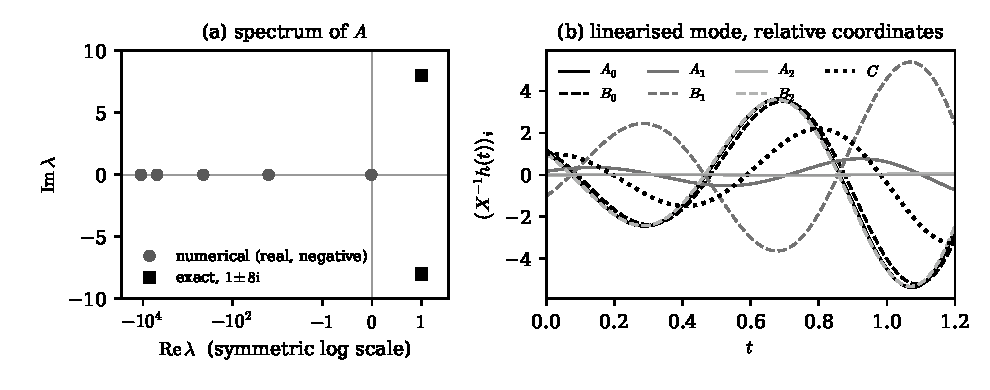
\includegraphics[width=\linewidth]{figures/spectrum.pdf}
\caption{(a) The seven eigenvalues of the Jacobian $A$: the exact pair $1\pm8\mathrm{i}$ (squares) and the five numerically computed real negative eigenvalues (circles), on a symmetric logarithmic real axis. (b) The exact linearised mode in relative coordinates, $X^{-1}h(t)=e^{t}(u\cos 8t-v\sin 8t)/200$, for $0\le t\le1.2$.}
\label{fig:spectrum}
\end{figure}

\subsection{Proof of Theorem~\ref{thm:main}}
Membership in the Type $\II_3$ family with unit weights and one subdivided return path, including source minimality, is Propositions~\ref{prop:minimal} and~\ref{prop:auto}. Positivity of the rates is~\eqref{eq:rates} with Table~\ref{tab:data}. Stationarity is Proposition~\ref{prop:stationary}, uniqueness is Proposition~\ref{prop:unique}, the eigenvalues $1\pm8\iu$ of the full Jacobian are Theorem~\ref{thm:eigenpair} together with Lemma~\ref{lem:jacobian}, and nonlinear instability with an oscillatory mode is Corollary~\ref{cor:instability}. \qed

\section{Mechanism and discovery}\label{sec:mechanism}

This section explains why the example exists and how it was found. Nothing here is used in the proof of Theorem~\ref{thm:main}; the numerical statements are labelled as such.

\subsection{Zero-frequency reduction is not dynamic reduction}\label{subsec:transfer}
Partition the Jacobian at a positive stationary state into the six retained species and the internal species $C$:
\[
A=\begin{pmatrix}J_{rr}&J_{ri}\\ J_{ir}&L\end{pmatrix},\qquad L\in\R .
\]
For $s\in\C$ with $s\ne L$, the eigenvalue equation $A\xi=s\xi$ with $\xi=(\xi_r,\xi_i)$ eliminates $\xi_i=(s-L)^{-1}J_{ir}\xi_r$ and becomes
\begin{equation}\label{eq:reduced}
\bigl(J_{rr}+J_{ri}(s-L)^{-1}J_{ir}\bigr)\xi_r=s\,\xi_r .
\end{equation}
At $s=0$ the matrix in~\eqref{eq:reduced} is the stationary Schur complement $J_{rr}-J_{ri}L^{-1}J_{ir}$, which is what any stationary contraction of the return path sees; this is the object controlled by the uniqueness and nonsingularity theorems of~\cite{TypeIIpos,TypeIImixed}. Stability, however, concerns~\eqref{eq:reduced} at every complex $s$. For the single intermediate of~\eqref{eq:network}, write the return path with its literal rate constants as
\[
B_0\ \overset{a}{\underset{b}{\rightleftarrows}}\ C\ \overset{c}{\underset{d}{\rightleftarrows}}\ A_1,\qquad C\xrightarrow{\ \delta\ }\varnothing,
\]
so that $\dot C=aB_0+dA_1-(b+c+\delta)C$ and $L=-(b+c+\delta)$. The internal block alone is stable. Its contribution to the two endpoint equations after elimination at frequency $s$ is
\begin{equation}\label{eq:transfer}
J_{ri}(s-L)^{-1}J_{ir}=\frac{1}{s+b+c+\delta}\begin{pmatrix}ab&bd\\ ac&cd\end{pmatrix}
\end{equation}
in the rows and columns of $(B_0,A_1)$. This is a first-order low-pass response with corner frequency $b+c+\delta$. For our parameters $b+c+\delta=k_1^-+k_6^++d_6\approx6.12$, while the growing mode has frequency $8$; at $s=8\iu$ the factor $(s+6.12)^{-1}$ has phase $-\arctan(8/6.12)\approx-52.6^\circ$ and modulus about $0.10$, whereas its zero-frequency value is real and about $0.16$. The return path therefore feeds the retained fork network with a delayed and attenuated version of the signal that the stationary contraction assumes to be instantaneous.

The consequence is visible numerically. The stationary Schur complement $J_{rr}-J_{ri}L^{-1}J_{ir}$ of our example has eigenvalues approximately $-0.0115$, $-1.90\pm12.8\iu$, $-451$, $-4859$, $-11202$: it is Hurwitz stable. The full seven-dimensional matrix is unstable with eigenvalues $1\pm8\iu$. Contracting $C$ at zero frequency turns the unstable oscillatory pair into a damped one and leaves everything else nearly unchanged. In the terminology of interconnected systems, a stable internal block and a stable zero-frequency contraction do not imply stability of the interconnection; the phase of the return response at the resonant frequency of the fork network is what matters. This is the precise sense in which the finite return paths permitted by the classification carry dynamical degrees of freedom that the stationary theory need not, and does not, control.

\subsection{How the example was found}\label{subsec:search}
The search proceeded in stationary coordinates throughout, so that every candidate was an actual positive stationary state of an actual rate assignment (Lemma~\ref{lem:coverage}), and the concentrations $x$ were free search variables, as Remark~\ref{rem:pencil} requires. Table~\ref{tab:search} summarises the steps; all runs were short.

\begin{table}[htbp]
\centering\small
\begin{tabular}{@{}>{\raggedright\arraybackslash}p{.30\linewidth}>{\raggedright\arraybackslash}p{.33\linewidth}>{\raggedright\arraybackslash}p{.30\linewidth}@{}}
\toprule
Step & Outcome & Conclusion drawn\\
\midrule
Diagonal Lyapunov metrics for the six-species stationary family (72 and 120 sampled cases) & Some metric searches failed; all sampled spectra were stable & A failed sufficient condition is not evidence of instability; test the spectrum directly\\
Concentration adversary on the failed-metric cases & No unstable spectrum & Failed metrics are poor seeds for instability\\
Return paths with 2, 4, 8 internal species matched to the same stationary Schur complement, on two stable seeds & Remained stable & Adding internal states is not automatically destabilising\\
Joint search over $(x,e,q)$ in the six-species family, minimising the angular damping $\Re\lambda/|\lambda|$ of the least damped complex pair & Best six-species case: $\Re\lambda/|\lambda|\approx-0.057$, pair $\approx-3.0\times10^{-4}\pm5.3\times10^{-3}\iu$ & A weakly damped asymmetric fork mode exists; use it as the seed\\
Return paths matched to that seed & $\Re\lambda/|\lambda|\approx+0.35$ with two internal species per return; larger with longer paths & First numerical instability\\
Reduction & One subdivided return with one internal species suffices; a coarse rational grid retained 87 unstable cases with strictly positive degradation & Seven species is the target\\
Exact design (Proposition~\ref{prop:linear}) & Prescribed $\lambda=1+8\iu$ and modal vector with denominator 200; strictly feasible rational vertex found in about two seconds & The certificate of Table~\ref{tab:data}\\
\bottomrule
\end{tabular}
\caption{The route to the certificate. Every numerical result here is discovery evidence only; the proof rests on Sections~\ref{sec:network}--\ref{sec:mode}.}
\label{tab:search}
\end{table}

Two choices were decisive. The first was the search objective. Several stable candidates had extremely slow real eigenvalues (the six-species seed also had a real eigenvalue near $-6\times10^{-8}$), so an objective based on the spectral abscissa is dominated by irrelevant slow relaxation. The angular damping $\Re\lambda/|\lambda|$ of a complex eigenvalue, which equals $-1$ for every negative real eigenvalue however small, isolates weakly damped \emph{oscillatory} modes, and it led directly to the seed. The second was to perturb the seed structurally, by giving a return link internal dynamics with the same zero-frequency response, rather than by enlarging the same random search; Section~\ref{subsec:transfer} explains why this is the perturbation the stationary theory does not see. The matched-path comparisons preserved the stationary Schur complement to roundoff ($10^{-13}$) and are numerical only; the final certificate does not depend on them.

\subsection{Exact spectral design is linear}\label{subsec:design}
The numerical candidate could have been certified by isolating a root of its seventh-degree characteristic polynomial in exact arithmetic. It was simpler, and more informative, to change the question.

\begin{proposition}[Linear exact design]\label{prop:linear}
Fix an invertible integer matrix $N$ with $P=I+N$, a vector $w\in\C^n$ and a number $\lambda\in\C$. The set of $(e,q,x)\in\R^{3n}$ such that the stationary coordinates $(q+N^{-1}e,\,q,\,e,\,x)$ satisfy
\begin{equation}\label{eq:design}
H(e,q)\,w=\lambda\,\diag(x)\,w,\qquad H(e,q)=-N\diag(q)N^{\mathsf T}+N\diag(N^{-1}e)-\diag(e),
\end{equation}
is a real linear subspace of $\R^{3n}$, cut out by $2n$ real linear equations. The admissibility conditions $e>0$, $q>0$, $x>0$, $q+N^{-1}e>0$ are strict linear inequalities. Hence, for rational $N$, $w$, $\lambda$, the existence of an admissible stationary state with eigenvalue $\lambda$ and relative eigenvector $w$ is a rational linear feasibility problem, and every feasible point yields a rational certificate.
\end{proposition}

\begin{proof}
$H(e,q)$ is linear in $(e,q)$ by~\eqref{eq:factor}, and $\diag(x)w$ is linear in $x$. Splitting~\eqref{eq:design} into real and imaginary parts gives $2n$ real linear equations. Lemma~\ref{lem:coverage} identifies the inequalities with admissibility. If the constraints are satisfiable, the strict feasible region is an open polyhedron in a rational subspace and contains rational points; the resulting $(p,q,e,x)$ are rational, and so are the rate constants~\eqref{eq:rates}.
\end{proof}

Discovery of the modal direction $w$ remains a nonlinear problem, but once a direction is chosen, certification is linear. For the example, the numerical unstable eigenvector of the seven-species candidate was converted to a relative vector $X^{-1}\xi$, rounded to the rational vector $(u+\iu v)/200$ of~\eqref{eq:uv}, and $\lambda$ was rounded to $1+8\iu$. A linear program with these constraints and a normalisation was strictly feasible; its active constraints were solved exactly in rational arithmetic, giving the vertex whose common denominator is the number $D$ of Table~\ref{tab:data}. Multiplying by $D$ gives the integer certificate, which leaves $A$ unchanged by Remark~\ref{rem:pencil}. A modal vector with denominator $1000$ was also feasible; it was not needed. Two remarks on the method: the vector that must be prescribed is the relative eigenvector $X^{-1}\xi$, not the physical one, because $x$ is unknown (a first attempt with the physical vector was discarded); and the rounding of $w$ is harmless because Proposition~\ref{prop:linear} is exact for whatever rational $w$ is chosen, the only risk being infeasibility, which did not occur.

\section{Formal verification}\label{sec:formal}

The example is compiled in Lean~4~\cite{dMU21}, version~4.30.0, against a frozen Mathlib~\cite{mathlib20} manifest with SHA-256
\begin{center}\small\texttt{a8df0b606ec258561c226df89856884be433c19b49fb0a27335d69bb2b6e9fac},\end{center}
the same environment as the companion papers~\cite{TypeIIpos,TypeIImixed}. The terminal declaration, in the namespace \lean{TypeIIStability}, is
\begin{lstlisting}
theorem typeII3_instability_counterexample :
    MixedDegradation.TypeII.PaperRaw.IsPaperTypeIILCore paperNetwork ∧
    paperNetwork.PositiveState paperState ∧
    paperNetwork.Stationary paperState ∧
    (∀ i, 0 < forwardRate i) ∧
    (∀ i, 0 < reverseRate i) ∧
    (∀ i, 0 < degradation i) ∧
    (∀ i, 0 < x i) ∧
    sourceDrift x = 0 ∧
    HasFDerivAt sourceDrift (MixedDegradation.matrixCLM A) x ∧
    DUnstableCores.HasEigenpair A (1 + 8 * Complex.I) eigenvector ∧
    DUnstableCores.HurwitzUnstable A
\end{lstlisting}
It has no hypotheses. A second declaration in the same file,
\begin{lstlisting}
theorem unique_positive_stationary_state (y : paperNetwork.State)
    (hy : paperNetwork.PositiveState y) (hs : paperNetwork.Stationary y) :
    y = paperState
\end{lstlisting}
instantiates the compiled Type $\II_\ell$ family theorem \lean{paper_typeII_l_unistationarity} of~\cite{TypeIImixed} on the same object \lean{paperNetwork}.

\subsection*{The interface}
\lean{paperNetwork} is a value of the type \lean{PaperRaw.OpenNetwork 3}, the literal weak-order source normal form of~\cite{TypeIIpos,TypeIImixed}: a Boolean weak-stem word (here all separated), a separated realisation with cyclic source partition, positive integer main weights (here all one), coefficient-one back products, a rate record with common positive forward and reverse constants and nonnegative degradation for every species, and literal reversible unit return chains of type \lean{UnitChain} (here of depths $1$, $2$, $1$, the middle one carrying the internal species $C$ with its own positive loss). \lean{IsPaperTypeIILCore} is the conjunction of $\Top$ and source minimality, the latter in the form that no proper weak-stem restriction retains $\Top$ and no rotated proper return cycle is stoichiometrically autocatalytic; \lean{PositiveState} and \lean{Stationary} are the literal positivity and mass-action balance conditions of the source model, including the balance at the internal species. \lean{sourceDrift} is the seven-dimensional vector field of the source model with the return state retained, and the module \lean{SourceDynamics} proves that it equals the literal polynomial field~\eqref{eq:field} at \emph{every} concentration vector, not only at $x$. \lean{HasFDerivAt} is Mathlib's Fr\'echet derivative; \lean{matrixCLM A} is the continuous linear map of the matrix $A=HX^{-1}$. \lean{HasEigenpair} $A\,\lambda\,\xi$ is the predicate $\xi\ne0$ and $A\xi=\lambda\xi$ with $A$ embedded entrywise in $\C$, and \lean{HurwitzUnstable A} asserts the existence of an eigenpair with $\Re\lambda>0$; both are inherited from an earlier development on unstable cores.

\subsection*{Module map}
Table~\ref{tab:modules} lists the modules under \lean{proofs/TypeIIStability/} and the statements of this paper they certify. The source-minimality proof in \lean{Source.lean} works on the contracted six-vertex skeleton with a small family of explicit reachability cuts, one for each omitted vertex and each fork, checked by kernel \lean{decide}, together with the unit-chain adapter for the return paths; Proposition~\ref{prop:minimal} is the equivalent direct seven-vertex argument. The derivative proof in \lean{PhysicalJacobian.lean} differentiates the relative-coordinate polynomial at $\one$ and composes with the positive diagonal map $z\mapsto X^{-1}z$, which is how the factorisation $A=HX^{-1}$ enters the formal statement. The eigenpair proof in \lean{Eigenpair.lean} uses only the two pencil identities of \lean{Witness.lean} and positivity of $x$.

\begin{table}[H]
\centering\small
\begin{tabular}{>{\raggedright\arraybackslash}p{.30\linewidth}>{\raggedright\arraybackslash}p{.64\linewidth}}
\toprule
Statement in this paper & Formal module and principal declarations\\
\midrule
Table~\ref{tab:data}, positivity; Proposition~\ref{prop:stationary}; Proposition~\ref{prop:pencil} & \lean{Witness.lean}: \lean{parameters_positive}, \lean{stationary_balance}, \lean{pencil_real}, \lean{pencil_imag}\\
Theorem~\ref{thm:eigenpair} & \lean{Eigenpair.lean}: \lean{eigenvector_ne_zero}, \lean{exact_eigenpair}, \lean{unstable}\\
Rates~\eqref{eq:rates}; field~\eqref{eq:field}; Lemma~\ref{lem:jacobian} at $x$ & \lean{PhysicalJacobian.lean}: \lean{rates_positive}, \lean{drift}, \lean{stationary}, \lean{physical_derivative}\\
Propositions~\ref{prop:minimal} and~\ref{prop:auto} (skeleton) & \lean{Source.lean}: \lean{skeleton}, \lean{avoid_certificate}, \lean{weak_minimal}, \lean{weak_top}\\
Membership, return chains, source stationarity & \lean{RawSource.lean}: \lean{paperNetwork}, \lean{returnChain}, \lean{unit_tail_minimal}, \lean{paper_core}, \lean{paper_positive}, \lean{paper_stationary}\\
Equality of the source field and~\eqref{eq:field} & \lean{SourceDynamics.lean}: \lean{source_drift_eq}, \lean{source_physical_derivative}\\
Theorem~\ref{thm:main} (spectral part); Proposition~\ref{prop:unique} & \lean{Resolution.lean}: \lean{typeII3_instability_counterexample}, \lean{unique_positive_stationary_state}\\
\bottomrule
\end{tabular}
\caption{Correspondence between the paper and the Lean development.}
\label{tab:modules}
\end{table}

\subsection*{Receipts}
The terminal module was checked with warnings treated as errors and exit code zero, in $94.5$ seconds, with all $93$ local dependency modules authenticated by source hash; the source of \lean{Resolution.lean} has SHA-256 \texttt{65f26f30\ldots0d08} and the authenticated elaborated type of the two declarations has fingerprint \texttt{sha256:12071a6d\ldots df79}. Both declarations report exactly the axioms \texttt{propext}, \texttt{Classical.choice} and \texttt{Quot.sound}, the standard foundation of Mathlib; there is no \texttt{sorry}, no native-computation axiom, and no assumed numerical certificate. The integer tables and both pencil identities of this paper were also replayed independently in exact rational arithmetic, together with the symbolic differentiation of~\eqref{eq:field} and the enumeration of Proposition~\ref{prop:minimal}; these replays guard against transcription errors and are not part of the formal evidence.

\subsection*{What is and is not formal}
The following are formal: source membership, including minimality, of the literal seven-species network; positivity and stationarity of $x$ in the source model; positivity of all rates; the vanishing of the full polynomial field at $x$; its Fr\'echet derivative $A$ at $x$; the eigenpair $(1+8\iu,\xi)$; Hurwitz instability of $A$; and uniqueness of the positive stationary state. The following are conventional: Lemmas~\ref{lem:coverage} and~\ref{lem:jacobian} as general statements (the formal development proves the derivative for the specific field), the linearised-instability theorem behind Corollary~\ref{cor:instability}, Proposition~\ref{prop:persist}, everything in Section~\ref{sec:mechanism}, and the identification of the source normal form with the prose classification of~\cite{NNU26}.

\section{Discussion}\label{sec:discussion}

\subsection*{What the example settles and what it leaves open}
Theorem~\ref{thm:main} answers negatively the question whether the unique positive stationary state of a source-minimal Type $\II_3$ core is Hurwitz stable for all positive rates and all positive degradation, when the cores are taken in the generality of the classification, with finite unit return paths. The finite return path is essential to this particular witness: in our bounded searches of the six-species subfamily in which every return link is a single reaction, the least damped complex pair reached an angular damping of about $-0.057$ but never crossed. Whether the six-species separated cores, or the three-species fully coincident Type $\II_3$ quotient, are always Hurwitz stable remains open. A positive answer would be a genuine composition statement: a network that is stable for all parameters becomes unstable for some parameters when one of its unit links is subdivided by an intermediate that is itself stable. Section~\ref{subsec:transfer} shows that such a statement would have to control the return response at nonzero frequency, not only at $s=0$.

\subsection*{Degradation as a bifurcation parameter}
Fix the reaction rate constants~\eqref{eq:rates} and consider the degradation vectors $\tau d$ for $\tau\in[0,1]$. At $\tau=0$ the reversible extension is detailed balanced and has a unique positive stationary state, which is Hurwitz stable; this persists for small $\tau$~\cite[Proposition~8.4]{TypeIImixed}. At $\tau=1$ the unique positive state is our $x$, which is unstable. If the positive stationary state exists for every $\tau\in[0,1]$, then it depends continuously on $\tau$ (the physical Jacobian is nonsingular at every positive stationary state by~\cite[Theorem~6.5 and Remark~8.3]{TypeIImixed}), and the spectrum, which starts in the open left half plane and ends with a pair at $1\pm8\iu$, must cross the imaginary axis at some $\tau_*\in(0,1)$ away from zero, since zero is excluded by nonsingularity. Such a crossing is a Hopf point if the crossing pair is simple and transversal, and the classical theory~\cite{Kuznetsov2004} would then give a branch of small periodic orbits. What is not known is whether the branch exists for every intermediate $\tau$: the uniqueness theorems are at-most-one statements, and the positive state may disappear at the origin or at infinity for some $\tau$~\cite[Proposition~8.5]{TypeIImixed} and reappear later.

\begin{question}\label{q:hopf}
For the rate constants~\eqref{eq:rates}, does the positive stationary state exist for all $\tau\in[0,1]$ along $\tau d$? If so, is the imaginary-axis crossing a nondegenerate Hopf bifurcation, and is the resulting periodic orbit stable?
\end{question}

The criteria of Vassena~\cite{Vassena2025Hopf} for Hopf bifurcation in mass-action systems without a Hurwitz computation, and the symbolic methods of~\cite{Vassena2024Symbolic}, are natural tools for the second part. A validated periodic orbit for a core with constant chemostats and linear degradation would be the first example of sustained oscillation in a minimal autocatalytic core in the strict sense of~\cite{NNU26}.

\subsection*{Relation to other notions of instability}
The example is an instability at one positive stationary state of one parameter assignment; it is not a parameter-independent structural statement. Structural theories of instability and oscillation in reaction networks, from the stoichiometric network analysis of Clarke~\cite{Clarke1980} to the graph-theoretic conditions of Mincheva and Roussel~\cite{MinchevaRoussel2007} and Angeli, Banaji and Pantea~\cite{AngeliBanajiPantea2014}, the unstable cores of Vassena and Stadler~\cite{VassenaStadler2024}, and the oscillatory cores of Blokhuis, Stadler and Vassena~\cite{BSV2025}, ask which networks admit instability for \emph{some} parameters, typically in the parameter-rich setting where kinetic derivatives are free. Our question is the opposite: the reversible extension of a core is a mass-action system with a fixed kinetic law, and the concern is whether its unique positive state can be unstable at all. The answer is yes, and the parameters realising it are rational and explicit. The autocatalysis-based oscillators of~\cite{BSV2025} are relevant comparisons, but their constructions use dynamic external reagents or catalytic degradation, which are not available in the literal setting here; the present example uses only the reversible extension and linear degradation. Among small bimolecular mass-action networks, the smallest admitting Hopf bifurcation were determined by Banaji and Boros~\cite{BanajiBoros2023}; our network is bimolecular, with seven species and twenty-one reactions including degradation, and it is not minimal in their sense, since minimality here is imposed by the core structure rather than by reaction count. Finally, the observation that $H$ is stable while $HX^{-1}$ is not is an instance of the failure of $D$-stability in the sense of the matrix-stability literature~\cite{Kushel2019}: on the stationary manifold the relevant question is whether the scaled Jacobian remains Hurwitz under all positive diagonal column scalings, and for cores with return intermediates it does not.

\subsection*{Detailed balance and deficiency}
At zero degradation the reversible extension is detailed balanced and its unique positive state is stable, in the setting of Horn and Jackson~\cite{HJ72} and the deficiency theory of Feinberg~\cite{Fei19}. Linear degradation destroys the complex-balanced structure. The uniqueness theorems~\cite{TypeIIpos,TypeIImixed} show that uniqueness survives this loss along every ray of degradation vectors; Theorem~\ref{thm:main} shows that stability does not. The two conclusions are not in tension: for the parameters of this paper the network has exactly one positive stationary state, and that state repels.

\subsection*{Open directions}
Beyond Question~\ref{q:hopf}, three directions seem worthwhile. First, a sufficient condition for stability of a Type $\II_\ell$ core with return paths that carries a transfer or storage property of each return module, of the kind~\eqref{eq:transfer}, rather than its stationary input--output relation; the matched-path experiments of Section~\ref{subsec:search} suggest that such a condition must involve the phase of the return response at the least damped frequency of the fork network. Second, the six-species question above, where the absence of an internal species removes the mechanism used here but where we have no stability proof. Third, the other families of the classification, for which the same stationary-coordinate search and the same linear exact-design step apply without change, since Lemma~\ref{lem:coverage} and Proposition~\ref{prop:linear} only require an invertible source matrix.

\section*{Acknowledgements}
To be inserted.

\bibliographystyle{plain}
\begingroup
\sloppy
\bibliography{refs}
\endgroup

\end{document}
